\documentclass[11pt,letterpaper,titlepage]{article}
\usepackage{fancyhdr}
\usepackage[left=0.75in, right=0.75in, bottom=1.0in]{geometry}
\usepackage{lastpage}
\usepackage{titleref}
\usepackage{booktabs}
\usepackage{appendix}
\appendixtitleon
\appendixtitletocon

\makeatletter

%================== List of figures and tables mods
\usepackage{tocloft}
\usepackage[labelfont=bf]{caption}

\renewcommand{\cftfigpresnum}{Figure\ }
\renewcommand{\cfttabpresnum}{Table\ }

\newlength{\mylenf}
\settowidth{\mylenf}{\cftfigpresnum}
\setlength{\cftfignumwidth}{\dimexpr\mylenf+1.5em}
\setlength{\cfttabnumwidth}{\dimexpr\mylenf+1.5em}


\newcommand{\half}{\frac{1}{2}}


%=================== Graphics
\usepackage{graphicx}
\usepackage[breakwords]{truncate}
\usepackage{float}
\usepackage{array}
\usepackage{amsmath}
\usepackage{mdframed}
\usepackage{fancyvrb}
\usepackage{float}
\usepackage{cancel}
\usepackage{amssymb}
\graphicspath{ {images/} }
\usepackage[usenames,dvipsnames,svgnames,table]{xcolor}
\usepackage[defaultlines=2,all]{nowidow}
\usepackage{listings}
\usepackage{color}
\definecolor{Brown}{cmyk}{0,0.81,1,0.60}
\definecolor{OliveGreen}{cmyk}{0.64,0,0.95,0.40}
\definecolor{CadetBlue}{cmyk}{0.62,0.57,0.23,0}
\usepackage{pdflscape}
\usepackage{relsize}
\usepackage{verbatim}
\usepackage{tabto}


%=================== Settings
\renewcommand{\baselinestretch}{1.2}
\definecolor{gray}{rgb}{0.4 0.4 0.4}
\newcommand{\stimes}{{\times}}

\begin{document}
\newcommand{\NSCDOCNUMBR}{NSC-REP-15-X}         %Put document number here
\newcommand{\NSCDOCSUBJT}{TECHNICAL REPORT: }   %Put document subject here
\newcommand{\NSCDOCTITLE}{$THERMOFLOW$ - System level Thermal-Hydraulics in $ChiTech$}       %Put document title here
\newcommand{\NSCDOCDATE} {March, 2016}    %Put document date here
\newcommand{\NSCDOCREV}  {Rev 1.01} %Put revision number here

\lstset{language=C++,frame=ltrb,framesep=4pt,basicstyle=\linespread{0.8} \small,
	keywordstyle=\ttfamily\color{OliveGreen},
	identifierstyle=\ttfamily\color{CadetBlue}\bfseries,
	commentstyle=\color{Brown},
	stringstyle=\ttfamily,
	showstringspaces=ture }


%################################# TITLE PAGE ########################
\begin{titlepage}
	\pagestyle{fancy}
	\vspace*{1.0cm}
	\centering
	%\includegraphics{NSC_Logo} \par
	\vspace{1cm}
	%\centering
	%{\Large\bfseries  \NSCDOCNUMBR   \par}
	\vspace{.25cm}
	%\centering
	{\Large\bfseries  \NSCDOCSUBJT \par} 
	{\Large\bfseries \NSCDOCTITLE  \par}
	\vspace{1cm}
	{\Large \NSCDOCDATE \par}
	\vspace{1.0cm}
	{\Large Jan Vermaak \& Guillermo Villanueva \par}
	{\Large \NSCDOCREV \par}
		
	\begin{comment}
	\renewcommand{\arraystretch}{2.0}
	\begin{tabular}{| m{2.5cm} | m{4.5cm} | m{4.5cm} |}
		\cline{2-3}
		\multicolumn{1}{c|}{} & \bfseries{Name} & \bfseries{Signature \& Date} \\ \hline
		\bfseries{Prepared} &     &     \\ \hline
		\bfseries{Reviewed} &     &     \\ \hline
		\bfseries{Reviewed} &     &     \\ \hline
	    \bfseries{Approved} &     &     \\ \hline
	\end{tabular} \par
	\end{comment}
	\begin{center}
		\begin{minipage}[c]{0.45\textwidth}
			\begin{figure}[H]
			
				
\includegraphics[width=3in]{Logo2_Medium.png}
			\end{figure}
		\end{minipage}
	\end{center}
	\vspace{2cm}
	%NSC-FRM-15-1 Rev.1
\end{titlepage}


\pagestyle{fancy}
\rfoot{Page \thepage \ of \pageref{LastPage}}
%\cfoot{NSC-FRM-15-1 Rev.1}
\cfoot{}
\lfoot{\truncate{14cm}{\NSCDOCTITLE}}
\rhead{}
\chead{\currentname}
\lhead{}
\renewcommand{\footrulewidth}{0.4pt}
\tableofcontents
\addtocontents{toc}{~\hfill\textbf{Page}\par}

\listoffigures
\listoftables
\chead{Contents}


\newpage
\chead{1 Conservation equations}
\section{Conservation equations}
The overall objective is that we want to solve the following four field variables:
\begin{itemize}
\item Pressure, $P$
\item Internal energy, $u$
\item Velocity, $v$
\item Density, $\rho$
\end{itemize}

\vspace{0.25cm}
\noindent
In order to do this we apply the conservation equations to the volume shown in Figure \ref{figure:ZZZ_ControlVolume} below:
	\begin{center}
		\begin{minipage}[c]{0.7\textwidth}
	
			\begin{figure}[H]
			
				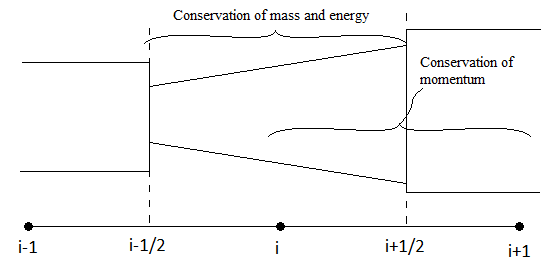
\includegraphics[width=5in]{ZZZ_ControlVolume.png}
				\caption{Simple layout of control volumes.}
				\label{figure:ZZZ_ControlVolume}
			\end{figure}
		\end{minipage}
	\end{center}
\vspace{0.5cm}

\newpage
\subsection{Conservation of Mass}
Even though we will be dealing with incompressible liquids, the liquids can exist at different temperatures and therefore different densities, $\rho$. The conservation of mass requires as a function of time, $t$:

\begin{equation*}
\frac{d\rho}{dt}=-\frac{1}{V}\int_S \rho.(\vec{v}\cdot \hat{n}).dA
\end{equation*}
\newline
\noindent And by applying it to the control volume:

\begin{equation}
\frac{d\rho_i}{dt} = \frac{1}{V_i}\biggr[ (\rho.A.v)_{i-\half}-(\rho.A.v)_{i+\half} \biggr]
\end{equation}

\noindent 
Where: 
\newline \noindent $v$ \quad = velocity.
\newline \noindent $V$ \quad = Volume.
\newline \noindent $A$ \quad = Area.
\newline \noindent $\hat{n}$ \quad = Surface normal.

\subsection{Conservation of Momentum}
The change in momentum, $\dot{m}_i.v_{i}$, in a control volume must balance the momentum of all the in and out flows as well as any forces applied:

\begin{equation*}
\frac{d}{dt}(\int_{CV}\rho.v.dV)+\int_S \rho.v.(\vec{v}\cdot \hat{n}).dA = \sum F_{cv}
\end{equation*}
\newline
\noindent For a control volume as shown in Figure \ref{figure:ZZZ_ControlVolume} we have:

\begin{equation}
\begin{aligned}
\frac{d(\rho_{i+\half}.v_{i+\half})}{dt}+ \frac{1}{V_{i+\half}} \biggr[   (\rho Av^2)_{i+1} - (\rho Av^2)_{i} \biggr]      &=-\frac{1}{V_{i+\half}} \biggr[   (PA)_{i+1}-(PA)_{i}  \biggr] +\rho_{i+\half}.g^* \\
&-\half \frac{1}{V_i}F_{\tau,i}-\half \frac{1}{V_{i+1}}F_{\tau,i+1}
\end{aligned}
\end{equation}
\newline
\noindent 
Where $V_{i+\half}=\half V_i+\half V_{i+1}$ is the distance between control volumes, $g^*$ is the gravitational force component (function of inclination angle between control volume centroids) and $F_{\tau}$ is the wall frictional force that can be calculated from the Darcy Friction Factor, $f$:

\begin{equation*}
F_{\tau}=\half f \rho \frac{L}{D} A v^2
\end{equation*} 
\noindent Therefore:

\begin{equation*}
\begin{aligned}
F_{\tau,i}&=\frac{1}{4} f_i \rho_i \frac{L_i}{D_i}A_i v_i^2 \\
F_{\tau,i+1}&=\frac{1}{4} f_{i+1} \rho_{i+1} \frac{L_{i+1}}{D_{i+1}}A_{i+1} v_{i+1}^2 \\
\end{aligned}
\end{equation*}
\newline
\noindent
In these equations $L_i$ and $D_i$ is the length and diameter of the $i$-th control volume


\subsection{Conservation of Energy}
The total energy of the system, $E$, must balance that of the in and out flow including the work performed and the heat transfer into the system:

\begin{equation*}
\frac{dE}{dt}=\int_S \rho.(\vec{v}\cdot \hat{n}).E.dA + Q - W -E_{loss}
\end{equation*}

\noindent 
Where: 
\newline \noindent $Q$ \quad = Heat transfer into the system.
\newline \noindent $W$ \quad = Work leaving the system.
\newline \noindent $E_{loss}$ \quad = Dissipative energy losses.
\newline
\newline
The components of energy are internal energy, $U$, kinetic energy, $\half mv^2$, and potential energy, $mgz$:

\begin{equation*}
E= m.e = m.(u+\half v^2+gz)
\end{equation*}
\newline
The heat transfer into the system is normally associated with some heat flux, $\dot{q}$, and the total heat transfer surface, $A_s$, therefore:

\begin{equation*}
Q_i=\dot{q}_i.A_{s,i}
\end{equation*}
\newline
The components of work include shaft work, $W_{shaft}$, and pressure work, $W_{pressure}$. For this case we will consider only pressure work:

\begin{equation*}
W_{pressure}=(P.A.v)_{i-\half} - (P.A.v)_{i+\half}
\end{equation*}
\newline
\noindent
From here the energy conservation equation becomes:

\begin{equation*}
\begin{aligned}
\frac{d}{dt} \biggr( m.(u+\half v^2+gz) \biggr)&=(\rho Av)_{i-\half}.(u+\half v^2+gz)_{i-\half} - (\rho Av)_{i+\half}.(u+\half v^2+gz)_{i+\half} \\
&+\dot{q}_i.A_{s,i} - \biggr[   (P.A.v)_{i-\half} - (P.A.v)_{i+\half}   \biggr] - E_{loss}
\end{aligned}
\end{equation*}
\newline
\noindent
Dividing by the volume we get:

\begin{equation}
\begin{aligned}
\frac{d}{dt} \biggr( \rho.(u+\half v^2) \biggr)&=\frac{1}{V_i}\biggr[ (\rho Av)_{i-\half}.(u+\half v^2+gz)_{i-\half} - (\rho Av)_{i+\half}.(u+\half v^2+gz)_{i+\half} \biggr] \\
&+\frac{A_{s,i}}{V_i}\dot{q}_i - \frac{1}{V_i}\biggr[   (P.A.v)_{i-\half} - (P.A.v)_{i+\half}   \biggr] - \frac{1}{V_i}E_{loss}
\end{aligned}
\end{equation}
\newline
\noindent The energy loss term includes both dynamic losses at the junctions and those within the control volume, however, for simplicity we will only consider the loss associated with junction losses for which the pressure loss is given by:

\begin{equation*}
\Delta P = \half K \rho  v^2
\end{equation*}
\newline
\noindent Where $K$ is a dimensionless parameter dependent on the geometry. The energy loss associated with this factor is:

\begin{equation*}
E_{loss,i-\half}=
\begin{cases}
(\Delta P.A.v)_{i-\half} = \half  K_{i-\half} (\rho A v^3)_{i-\half}     &,v_{i-\half}>0 \\
0    &,v_{i-\half}<0
\end{cases}
\end{equation*}
\newline
\noindent Similarly:
\begin{equation*}
E_{loss,i+\half}=
\begin{cases}
(\Delta P.A.v)_{i+\half} = \half  K_{i+\half} (\rho A v^3)_{i+\half}     &,v_{i+\half}<0 \\
0    &,v_{i+\half}>0
\end{cases}
\end{equation*}


\subsection{Equation of state}
In addition to the conservation equations, there is the equation of state. For the incompressible liquids of this simulation we can approximate the equation of state as:

\begin{equation}
\begin{aligned}
u&=-0.002053148 \ \rho^3+5.927524805 \ \rho^2-5710.176493 \ \rho+1835863.516 \\
\rho&=7.88656E-06 \ T^3-0.004477273 \ T^2-0.059652292 \ T+1001.25303
\end{aligned}
\end{equation}





\newpage
\chead{2 Numerical solution}
\section{Numerical solution}
The conservation of momentum equations conveniently couples the pressure field and velocities and therefore is used implicitly to determine the pressures at time $n+1$.

\subsection{Conservation of Mass - finite difference formulation}
The finite difference formulation is as follows:


\begin{equation*}
\frac{\rho_i^{n+1} - \rho_i^{n}}{\Delta t} = \frac{1}{V_i}\biggr[ (\rho.A.v)_{i-\half}^{n}-(\rho.A.v)_{i+\half}^{n} \biggr]
\end{equation*}

\noindent Therefore we get:

\begin{equation}
\rho_i^{n+1}  = \rho_i^{n}+\frac{\Delta t}{V_i}\biggr[ (\rho.A.v)_{i-\half}^{n}-(\rho.A.v)_{i+\half}^{n} \biggr]
\end{equation}




\subsection{Conservation of Momentum - finite difference formulation}
Because no other future time equation has pressure as a variable we opt to include pressure at time $n+1$ as an implicit variable. We manipulate the original conservation of mass equation:
\begin{equation*}
\begin{aligned}
\frac{d(\rho_{i+\half}.v_{i+\half})}{dt}+ \frac{1}{V_{i+\half}} \biggr[   (\rho^*Av^2)_{i+1} - (\rho^*Av^2)_{i} \biggr]      &=-\frac{1}{V_{i+\half}} \biggr[   (PA)_{i+1}-(PA)_{i}  \biggr] +\rho_{i+\half}.g^* \\
&-\half \frac{1}{V_i}F_{\tau,i}-\half \frac{1}{V_{i+1}}F_{\tau,i+1}
\end{aligned}
\end{equation*}

\noindent We use the following time notation:

\begin{equation*}
\begin{aligned}
\rho_{i+\half}^{n+1}.v_{i+\half}^{n+1}-\rho_{i+\half}^n.v_{i+\half}^n+ \frac{\Delta t}{V_{i+\half}} \biggr[   (\rho Av^2)_{i+1}^n - (\rho Av^2)_{i}^n \biggr]      &=-\frac{\Delta t}{V_{i+\half}} \biggr[   (PA)_{i+1}^{n+1}-(PA)_{i}^{n+1}  \biggr] +\rho_{i+\half}^n.g^*\Delta t \\
&-\half \frac{\Delta t}{V_i}F_{\tau,i}^n-\half \frac{\Delta t}{V_{i+1}}F_{\tau,i+1}^n
\end{aligned}
\end{equation*}
\newline
\noindent And rearrange the terms:

\begin{equation}
\begin{aligned}
\rho_{i+\half}^{n+1}.v_{i+\half}^{n+1} +\frac{\Delta t}{V_{i+\half}} \biggr[   (PA)_{i+1}^{n+1}-(PA)_{i}^{n+1}  \biggr]     &=\rho_{i+\half}^n.v_{i+\half}^n - \frac{\Delta t}{V_{i+\half}} \biggr[   (\rho Av^2)_{i+1}^n - (\rho Av^2)_{i}^n \biggr]\\
& +\rho_{i+\half}^n.g^*\Delta t -\half \frac{\Delta t}{V_i}F_{\tau,i}^n-\half \frac{\Delta t}{V_{i+1}}F_{\tau,i+1}^n\\
\end{aligned}
\end{equation}
\newline
\noindent In the equations above we included implicit time instances to pressure in order to semi-implicitly couple the system.




\subsection{Conservation of Energy - finite difference formulation}
We start with the original conservation of energy equation:

\begin{equation*}
\begin{aligned}
\frac{d}{dt} \biggr( \rho.(u+\half v^2) \biggr)&=\frac{1}{V_i}\biggr[ (\rho Av)_{i-\half}.(u+\half v^2+gz)_{i-\half} - (\rho Av)_{i+\half}.(u+\half v^2+gz)_{i+\half} \biggr] \\
&+\frac{A_{s,i}}{V_i}\dot{q}_i - \frac{1}{V_i}\biggr[   (P.A.v)_{i-\half} - (P.A.v)_{i+\half}   \biggr] - \frac{1}{V_i}E_{loss}
\end{aligned}
\end{equation*}
\newline
\noindent We now discretize the left side and set the right side to correspond to time $n$.

\begin{equation*}
\begin{aligned}
\frac{(\rho_i^{n+1}.u_i^{n+1}-  \rho_i^{n}.u_i^{n}) + (\half.\rho_i^{n+1}.(v_i^{n+1})^2   -\half.\rho_i^{n}.(v_i^{n})^2)}{\Delta t}&=\frac{1}{V_i}\biggr[ (\rho Av)_{i-\half}^n.(u+\half v^2+gz)_{i-\half}^n \\
&- (\rho Av)_{i+\half}^n.(u+\half v^2+gz)_{i+\half}^n \biggr] \\
&+\frac{A_{s,i}}{V_i}\dot{q}_i^n - \frac{1}{V_i}\biggr[   (P.A.v)_{i-\half}^n - (P.A.v)_{i+\half}^n   \biggr] \\
&- \frac{1}{V_i}E_{loss}^n
\end{aligned}
\end{equation*}
\newline
\noindent And finally:

\begin{equation}
\begin{aligned}
\rho_i^{n+1}.u_i^{n+1} + \half.\rho_i^{n+1}.(v_i^{n+1})^2 &=\rho_i^{n}.u_i^{n} +\half.\rho_i^{n}.(v_i^{n})^2+ \frac{1}{V_i}\biggr[ (\rho Av)_{i-\half}^n.(u+\half v^2+gz)_{i-\half}^n \\
&- (\rho Av)_{i+\half}^n.(u+\half v^2+gz)_{i+\half}^n \biggr] \\
&+\frac{A_{s,i}}{V_i}\dot{q}_i^n - \frac{1}{V_i}\biggr[   (P.A.v)_{i-\half}^n - (P.A.v)_{i+\half}^n   \biggr] \\
&- \frac{1}{V_i}E_{loss}^n
\end{aligned}
\end{equation}






\subsection{Unknowns in the available equations}
The "new" time values that require solving are found in the following left hand terms:

\begin{equation*}
\begin{aligned}
&\rho_i^{n+1} \\
&\rho_{i+\half}^{n+1}.v_{i+\half}^{n+1} +\frac{\Delta t}{V_{i+\half}} \biggr[   (PA)_{i+1}^{n+1}-(PA)_{i}^{n+1}  \biggr]    \\
&\rho_i^{n+1}.u_i^{n+1} + \half.\rho_i^{n+1}.(v_i^{n+1})^2
\end{aligned}
\end{equation*}
\newline
We change $\rho_{i+\half}^{n+1}$ according to:

\begin{equation*}
\rho_{i+\half}^{n+1}=
\begin{cases}
\rho_{i}^{n+1}       &, v_{i+\half}>0 \\
\rho_{i+1}^{n+1}     &, v_{i+\half}<0
\end{cases}
\end{equation*}
\newline
We then change $v_i^{n+1}$ according to $v_{i+\half}^{n+1}\frac{A_{i+\half}}{A_i}$. A "thing" that will be tested later but will allow us to determine $v_{i+\half}$ from equation 7.




\subsection{Semi-implicit approach}
From equation 5 we can solve for $\rho_i^{n+1}$ and from equation 4 we can solve for $u_i^{n+1}$. From equation 7 we can solve for $v_{i+\half}^{n+1}$. Now the only variables left unsolved is the pressures $P_{i+1}^{n+1}$ and $P_{i}^{n+1}$.
\newline
\newline
Hence we are left with the conservation of momentum equation with the unknowns $P_{i}$ and $P_{i+1}$. Therefore, in a single time step where we have $I$ amount of control volumes as shown in Figure \ref{figure:ZZZ_SimpleSystem} below, we will have $I$ unknowns and $I$ amount of momentum equations. 

	\begin{center}
		\begin{minipage}[c]{0.85\textwidth}
	
			\begin{figure}[H]
			
				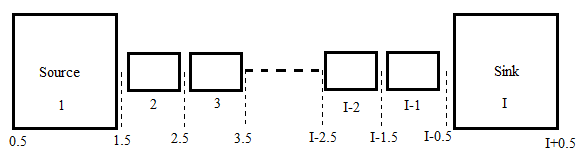
\includegraphics[width=6in]{ZZZ_SimpleSystem.png}
				\caption{Simple layout of multiple control volumes.}
				\label{figure:ZZZ_SimpleSystem}
			\end{figure}
		\end{minipage}
	\end{center}
\vspace{0.5cm}










\newpage
\subsection{Solution algorithm}

\textbf{Step 1}\newline
Load all control volumes. Input parameters:
\begin{itemize}
\item Area, $A$
\item Length, $L$
\item Pressure, $P$
\item Temperature, $T$
\item Elevation change, $\Delta z$
\item Wall roughness, $\epsilon$
\end{itemize}
\vspace{0.25cm}
Determine density, $\rho_i$, from:

\begin{equation*}
\rho=7.88656E-06 \ T^3-0.004477273 \ T^2-0.059652292 \ T+1001.25303
\end{equation*}
\newline
And internal energy from:
\begin{equation*}
u=-0.002053148 \ \rho^3+5.927524805 \ \rho^2-5710.176493 \ \rho+1835863.516 
\end{equation*}



\vspace{0.5cm}\noindent
\textbf{Step 2}\newline
Load all junctions. Input parameters:
\begin{itemize}
\item Junction velocity, $v$
\item Area, $A$
\item Loss factor, $K$
\end{itemize}

\noindent Determine all junction $z$ values using control volume $\Delta z$ values.




\vspace{0.5cm}\noindent
\textbf{Step 3}\newline
Determine $\rho_{i-\half}^n$ and $\rho_{i+\half}^n$ as follows:
\begin{equation*}
\rho_{i-\half}^n=
\begin{cases}
\rho_{i-1}^n     &,v_{i-\half}>0 \\
\rho_{i}^n    &,v_{i-\half}<0
\end{cases}
\end{equation*}
\begin{equation*}
\rho_{i+\half}^n=
\begin{cases}
\rho_{i}^n     &,v_{i+\half}>0 \\
\rho_{i+1}^n    &,v_{i+\half}<0
\end{cases}
\end{equation*}
And similarly for $u_{i-\half}^n$ and $u_{i+\half}$ from:
\begin{equation*}
u_{i-\half}^n=
\begin{cases}
u_{i-1}^n     &,v_{i-\half}>0 \\
u_{i}^n    &,v_{i-\half}<0
\end{cases}
\end{equation*}
\begin{equation*}
u_{i+\half}^n=
\begin{cases}
u_{i}^n     &,v_{i+\half}>0 \\
u_{i+1}^n    &,v_{i+\half}<0
\end{cases}
\end{equation*}



\vspace{0.5cm}\noindent
\textbf{Step 4}\newline
Run through each control volume and apply equation 5:

\begin{equation*}
\rho_i^{n+1}  = \rho_i^{n}+\frac{\Delta t}{V_i}\biggr[ (\rho.A.v)_{i-\half}^{n}-(\rho.A.v)_{i+\half}^{n} \biggr]
\end{equation*}



\vspace{0.5cm}\noindent
\textbf{Step 5}\newline
Determine internal energy, $u^{n+1}$, using density, $\rho^{n+1}$ from equation 4:
\begin{equation*}
u=-0.002053148 \ \rho^3+5.927524805 \ \rho^2-5710.176493 \ \rho+1835863.516 
\end{equation*}







\vspace{0.5cm}\noindent
\textbf{Step 6}\newline
Determine the elements of equation 7:
\begin{equation*}
\begin{aligned}
\rho_i^{n+1}.u_i^{n+1} + \half.\rho_i^{n+1}.(v_{i+\half}^{n+1}\frac{A_{i+\half}}{A_i})^2 &=\rho_i^{n}.u_i^{n} +\half.\rho_i^{n}.(v_{i+\half}^{n}\frac{A_{i+\half}}{A_i})^2+ \frac{1}{V_i}\biggr[ (\rho Av)_{i-\half}^n.(u+\half v^2+gz)_{i-\half}^n \\
&- (\rho Av)_{i+\half}^n.(u+\half v^2+gz)_{i+\half}^n \biggr] \\
&+\frac{A_{s,i}}{V_i}\dot{q}_i^n - \frac{1}{V_i}\biggr[   (P.A.v)_{i-\half}^n - (P.A.v)_{i+\half}^n   \biggr] \\
&- \frac{1}{V_i}E_{loss}^n
\end{aligned}
\end{equation*}
In elemental form we want to determine $v_{i+\half}^{n+1}$ from:
\begin{equation*}
\begin{aligned}
J + M(v_{i+\half}^{n+1}N)^2 &=B+\frac{1}{V_i}\biggr[ C - D \biggr]+E - \frac{1}{V_i}\biggr[   F - G   \biggr]- H
\end{aligned}
\end{equation*}
Where:
\begin{equation*}
\begin{aligned}
B&=\rho_i^{n}.u_i^{n} +\half.\rho_i^{n}.(v_{i+\half}^{n}\frac{A_{i+\half}}{A_i})^2 \\
C&=(\rho Av)_{i-\half}^n.(u+\half v^2+gz)_{i-\half}^n\\
D&=(\rho Av)_{i+\half}^n.(u+\half v^2+gz)_{i+\half}^n\\
E&=\frac{A_{s,i}}{V_i}\dot{q}_i^n \quad F=P_{i}^n(A.v)_{i-\half}^n \quad G=P_{i}^n(A.v)_{i+\half}^n\\
H&=\frac{1}{V_i}E_{loss}^n \quad J=\rho_i^{n+1}.u_i^{n+1} \quad M=\half.\rho_i^{n+1} \quad N=\frac{A_{i+\half}}{A_i}\\
\end{aligned}
\end{equation*}
\newline
The $P_{i-\half}$ terms in these elements were exchanged with $P_i$ terms. This is a valid approximation since $P_i-P_{i-\half}\approx P_{i+\half}-P_i$. The $E_{loss}^n$ term needs to be calculated as follows:
\begin{equation*}
E_{loss}^n=E_{loss,i+\half}^n+E_{loss,i-\half}^n
\end{equation*}
Where:
\begin{equation*}
E_{loss,i-\half}=
\begin{cases}
(\Delta P.A.v)_{i-\half} = \half  K_{i-\half} (\rho A v^3)_{i-\half}^n     &,v_{i-\half}>0 \\
0    &,v_{i-\half}<0
\end{cases}
\end{equation*}
\newline
\noindent And:
\begin{equation*}
E_{loss,i+\half}=
\begin{cases}
(\Delta P.A.v)_{i+\half} = \half  K_{i+\half} (\rho A v^3)_{i+\half}^n     &,v_{i+\half}<0 \\
0    &,v_{i+\half}>0
\end{cases}
\end{equation*}
\newline
Then calculate:
\begin{equation*}
\begin{aligned}
B_1&= B+\frac{1}{V_i}\biggr[ C - D \biggr]+E - \frac{1}{V_i}\biggr[   F - G   \biggr]- H-J \\
B_2&=\sqrt{\frac{B_1}{M}}
\end{aligned}
\end{equation*}
And finally:
\begin{equation*}
v_{i+\half}^{n+1}=\frac{B_2}{N}
\end{equation*}



\vspace{0.5cm}\noindent
\textbf{Step 6}\newline
Preparing for step 7 we set:
\begin{equation*}
\rho_{i+\half}^{n+1}=
\begin{cases}
\rho_{i}^{n+1}     &,v_{i+\half}^{n+1}>0 \\
\rho_{i+1}^{n+1}    &,v_{i+\half}^{n+1}<0
\end{cases}
\end{equation*}
And we calculate the arithmetic average volume velocity:
\begin{equation*}
v_i^n = \frac{(Av)_{i-\half}+(Av)_{i+\half}}{2.A_i}
\end{equation*}


\newpage
\noindent
\textbf{Step 7}\newline
Determine the elements of equation 6:
\begin{equation*}
\begin{aligned}
\rho_{i+\half}^{n+1}.v_{i+\half}^{n+1} +\frac{\Delta t}{V_{i+\half}} \biggr[   (PA)_{i+1}^{n+1}-(PA)_{i}^{n+1}  \biggr]     &=\rho_{i+\half}^n.v_{i+\half}^n - \frac{\Delta t}{V_{i+\half}} \biggr[   (\rho Av^2)_{i+1}^n - (\rho Av^2)_{i}^n \biggr]\\
& +\rho_{i+\half}^n.g^*\Delta t -\half \frac{\Delta t}{V_i}F_{\tau,i}^n-\half \frac{\Delta t}{V_{i+1}}F_{\tau,i+1}^n\\
\end{aligned}
\end{equation*}
In elemental form:
\begin{equation*}
\begin{aligned}
H +\frac{\Delta t}{V_{i+\half}} \biggr[   (PA)_{i+1}^{n+1}-(PA)_{i}^{n+1}  \biggr]     &=B - \frac{\Delta t}{V_{i+\half}} \biggr[   C - D \biggr] +E -F-G\\
\end{aligned}
\end{equation*}
Where:
\begin{equation*}
\begin{aligned}
B&=\rho_{i+\half}^n.v_{i+\half}^n  \quad C=(\rho Av^2)_{i+1}^n  \quad D=(\rho Av^2)_{i}^n  \quad E=\rho_{i+\half}^n.g^*\Delta t \\ 
F&=\half \frac{\Delta t}{V_i}F_{\tau,i}^n  \quad G=\half \frac{\Delta t}{V_{i+1}}F_{\tau,i+1}^n  \quad
H=\rho_{i+\half}^{n+1}.v_{i+\half}^{n+1}
\end{aligned}
\end{equation*}
\newline
In order to calculate $F_{\tau,i}^n$ and $F_{\tau,i+1}^n$ we need to apply the following:

\begin{equation*}
\begin{aligned}
F_{\tau,i}^n&=\frac{1}{4} f_i^n \rho_i^n \frac{L_i^n}{D_i^n}A_i^n (v_i^n)^2 \\
F_{\tau,i+1}^n&=\frac{1}{4} f_{i+1}^n \rho_{i+1}^n \frac{L_{i+1}^n}{D_{i+1}^n}A_{i+1}^n (v_{i+1}^n)^2 \\
\end{aligned}
\end{equation*}
\newline
Where $f_{i}^n$ and $f_{i+1}^n$ are calculated from the transcendental equation:
\begin{equation*}
\frac{1}{\sqrt{f}}=-2 \ \mathrm{log} \biggr ( \frac{\epsilon}{3.7 D_h}+\frac{2.51}{Re \sqrt{f}}    \biggr)
\end{equation*}
\newline
Where $Re$ is the dimensionless Reynold's number defined as:
\begin{equation*}
Re=\frac{\rho_i^n v_i^n D_h}{\mu_i^n}
\end{equation*}
\newline
Now calculate the equation in its final form calculate:
\begin{equation*}
\begin{aligned}
A_{1,i}&=\frac{\Delta t A_{i}}{V_{i+\half}} \\
A_{2,i}&=\frac{\Delta t A_{i+1}}{V_{i+\half}} \\
B_{i}&=B - \frac{\Delta t}{V_{i+\half}} \biggr[   C - D \biggr] +E -F-G-H\\
\end{aligned}
\end{equation*}
\newline
Now one can construct a linear system $Ax=b$ with elements:
\begin{equation*}
A_{j,i}=
\begin{cases}
A_{1,j}                  &, i=j \\
A_{2,j}                  &, i=j+1 \\
0                   &, i<j \ and \ i>j+1
\end{cases}
\end{equation*}
\begin{equation*}
x=[P_1 \ P_2 \ \dots \ P_{i-1} \ P_i]^T
\end{equation*}
\begin{equation*}
b=[b_1 \ b_2 \ \dots \ b_{i-1} \ b_i]^T, \quad \ b_j=B_i
\end{equation*}
\newline
This system is a diagonal system of unknowns and can be solved by any suitable solver.

\newpage
\chead{References}
\begin{thebibliography}{1}

	\bibitem{NUREG1282} {\em Safety Evaluation Report on High-Uranium Content, Low-Enriched Uranium-Zirconium Hydride Fuels for TRIGA Reactors}, NUREG-1282, Docket number 50-163, GA Technologies, August 1987.
	
	\bibitem{CpUranium} Ginnings D.C., Corruccini R.J., {\em Heat Capacities at High Temperatures of Uranium, Uranium Trichloride, and Uranium Tetrachloride}, Journal of Research of the National Bureau of Standards, Research Paper RP1831, Volume 39, October 1947.
	
	\bibitem{CpZircHydride} Douglas T.B., Victor A.C., {\em Heat Content of Zirconium and of Five Compositions of Zirconium Hydride from $0^{\circ}$ to $990^{\circ}C$}, Journal of Research of the National Bureau of Standards, Research Paper RP2878, Volume 61, July 1958.
	
\end{thebibliography}





\end{document}